% ============================================================================
% Appendix D: Extended Experimental Results
% Contains content demoted from main body for focus
% ============================================================================

\section{Extended Experimental Results}
\label{app:adaptation_details}

This appendix provides full experimental details, figures, and extended analysis for the adaptation and robustness results summarized in Section~\ref{sec:robustness_adaptation}.

% ----------------------------------------------------------------------------
% D.1: Distribution Shift Visualization
% ----------------------------------------------------------------------------

\subsection{Distribution Shift Analysis}
\label{app:distribution_shift}

Figure~\ref{fig:distribution_shift} provides the full visualization of the covariate shift between offline training and holdout evaluation distributions, summarized quantitatively in Section~\ref{sec:distribution_shift}. As noted in the main text, this shift reflects heterogeneity between two different data collections (RouteLLM battles vs.\ LMSYS dev/holdout) rather than a measured production drift.

\begin{figure}[h]
\centering
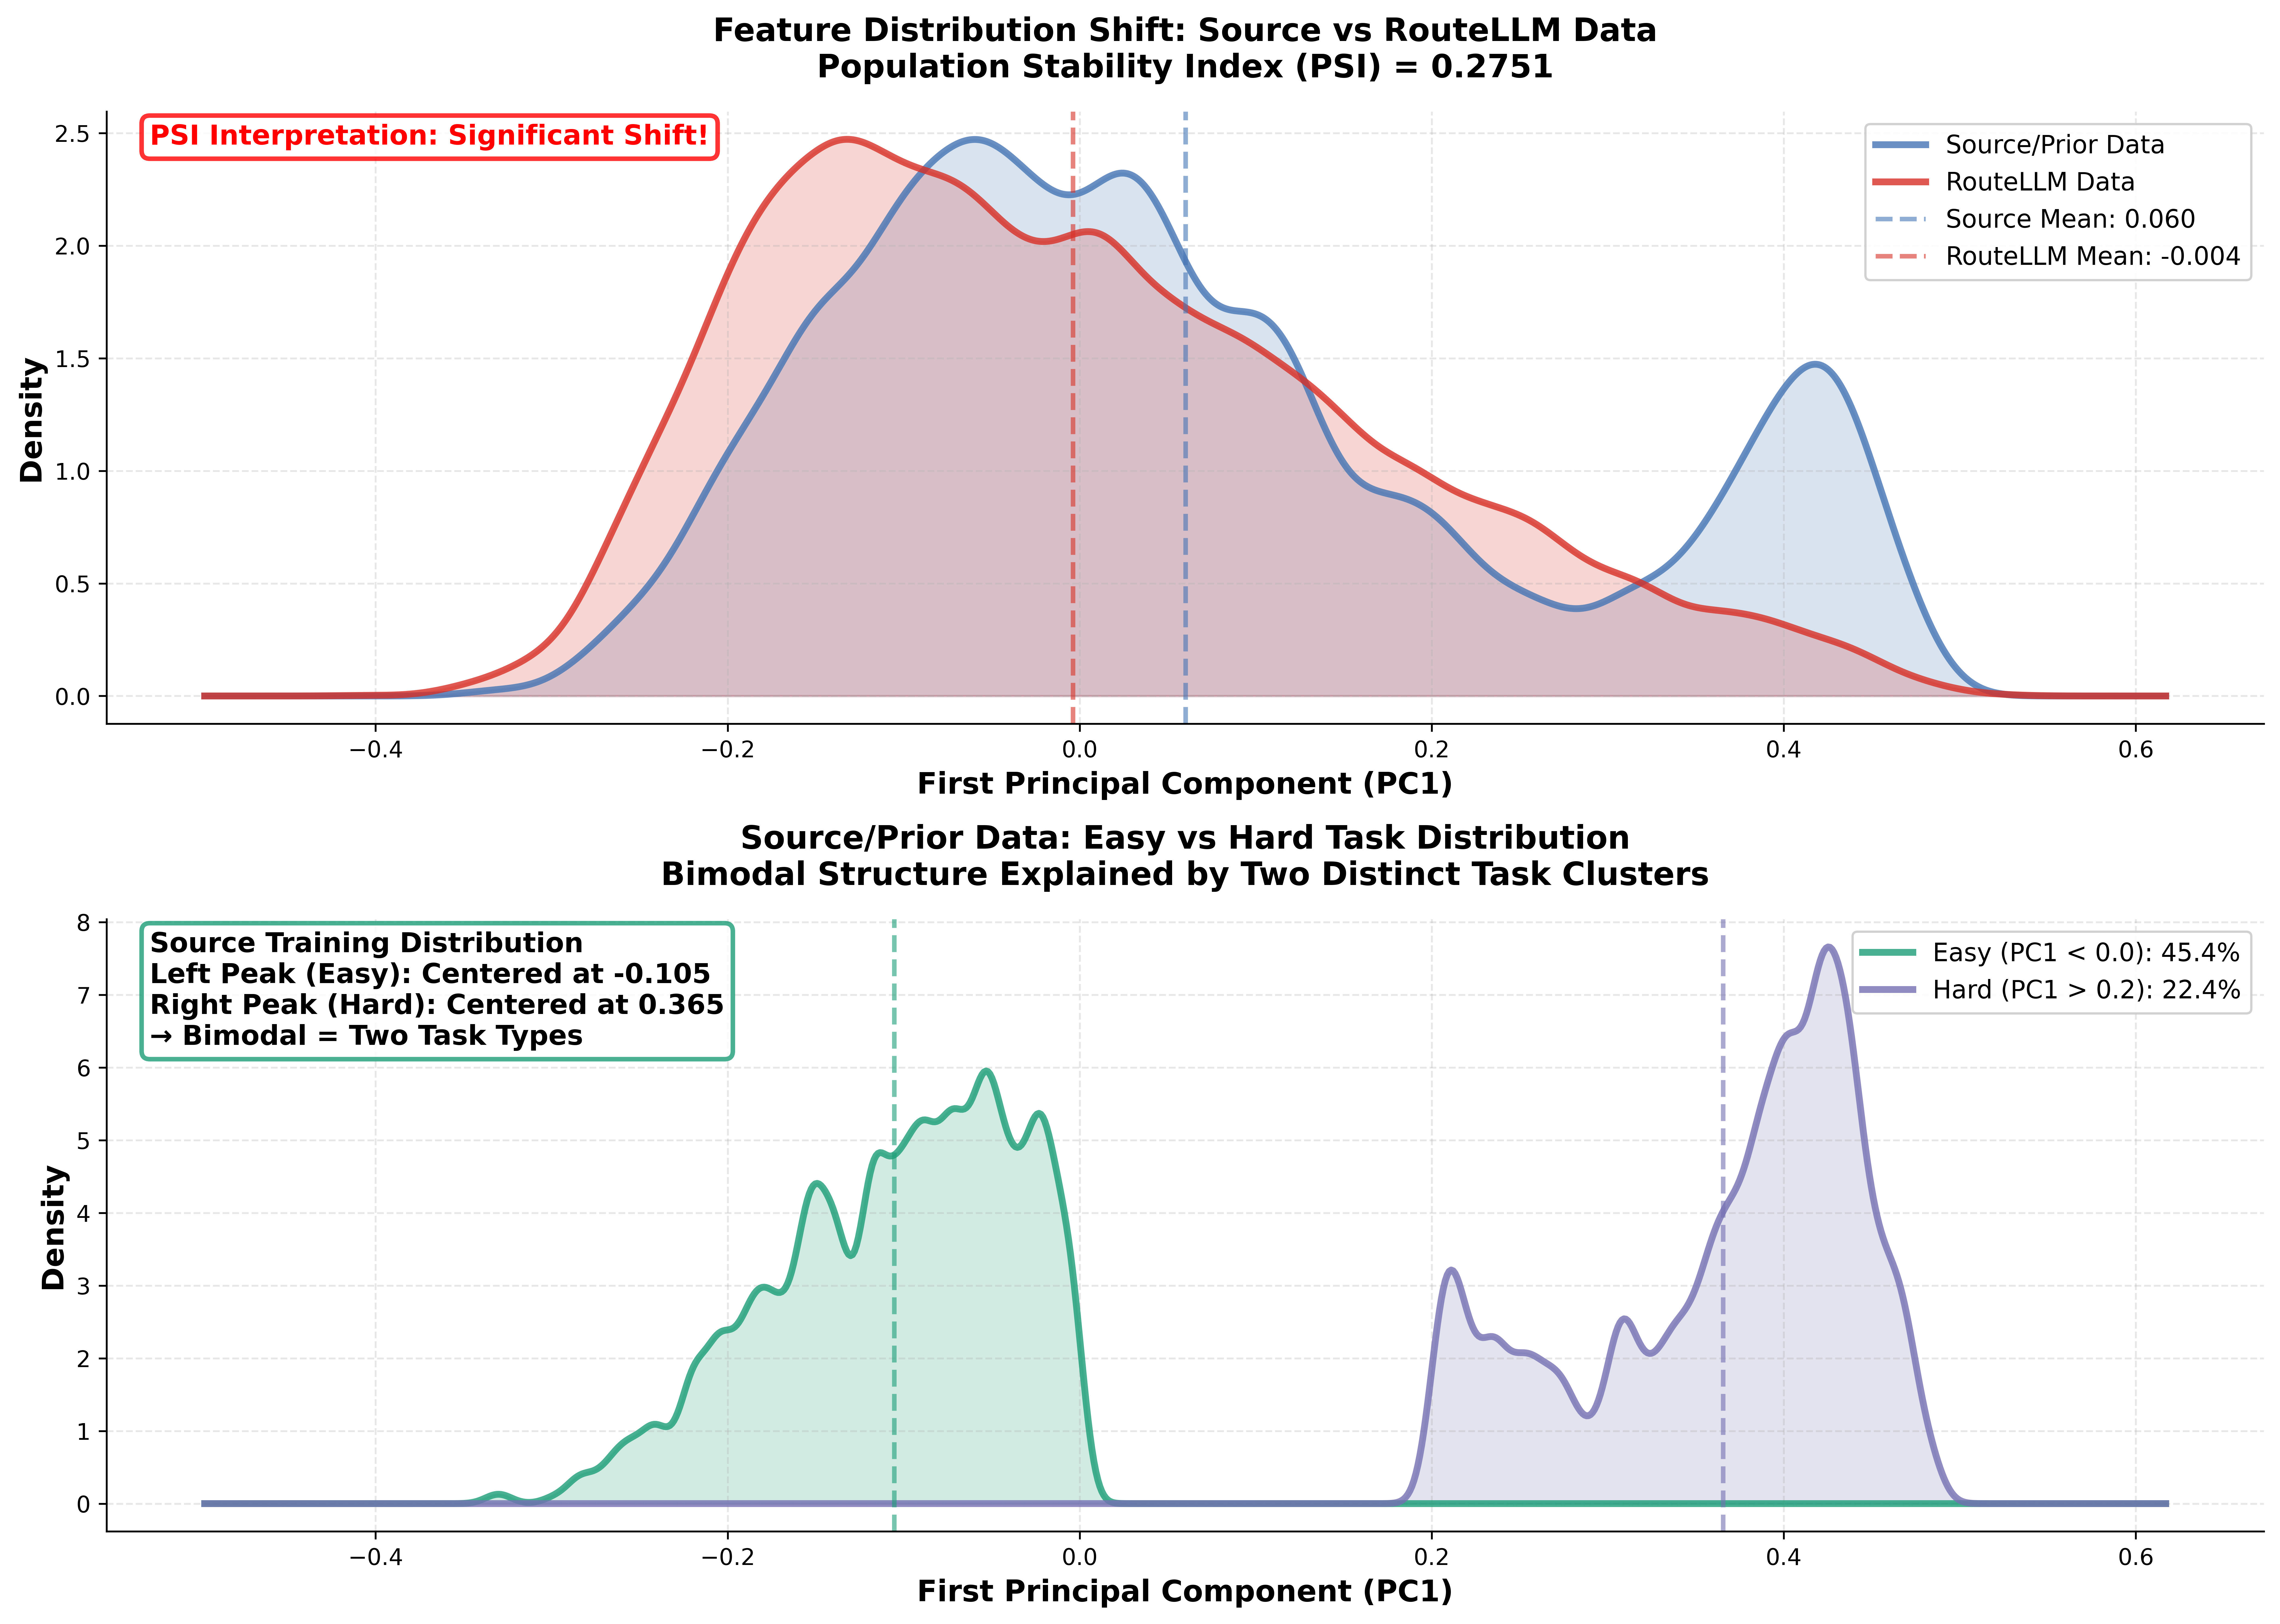
\includegraphics[width=0.9\columnwidth]{figures/figure2_distribution_shift.png}
\caption{\textbf{Distribution Shift Visualization.}
\textbf{Top:} Density comparison (PSI = 0.275) shows a structural mismatch between Offline Training priors (Blue) and Holdout evaluation data (Red) in the PC1 feature space.
\textbf{Bottom:} Decomposition based on the reward gap zones from Table~\ref{tab:cluster_inversion}. The Alignment Tax Cluster (Right Peak, PC1 $>$ 0.3, where Mixtral wins with $\Delta = -0.68$) is over-represented in offline data. The Natural Language Cluster (Left Peak, PC1 $<$ 0.3, where GPT-4 wins with $\Delta = +0.13$) dominates production traffic.
The Offline Prior over-indexes on the Alignment Tax cluster, leading to systematic underestimation of GPT-4's utility on dominant Natural Language traffic.}
\label{fig:distribution_shift}
\end{figure}

\paragraph{Forensic Decomposition.}
The shift decomposes into two functional zones aligned with the Alignment Tax discovery:
\begin{enumerate}[nosep]
    \item \textbf{Natural Language Zone (PC1 $< 0.3$):} Open-ended chat where GPT-4's nuance yields a positive advantage ($\Delta = +0.13$).
    \item \textbf{Alignment Tax Zone (PC1 $\geq 0.3$):} Strict constraints where GPT-4's alignment artifacts cause failure ($\Delta = -0.68$).
\end{enumerate}

Offline data is heavily weighted toward the Alignment Tax zone, while the holdout evaluation set is dominated by the Natural Language zone. This directional mismatch means a static router trained on offline data systematically under-provisions GPT-4 on evaluation traffic---the ``False Negative'' policy described in Section~\ref{sec:distribution_shift}.

% ----------------------------------------------------------------------------
% D.2: Catastrophic Failure Detection
% ----------------------------------------------------------------------------

\subsection{Catastrophic Failure Detection}
\label{app:catastrophic_failure}

Figure~\ref{fig:decommission} visualizes the internal dynamics of our Corralling Algorithm handling catastrophic model degradation.

\begin{figure}[h]
\centering
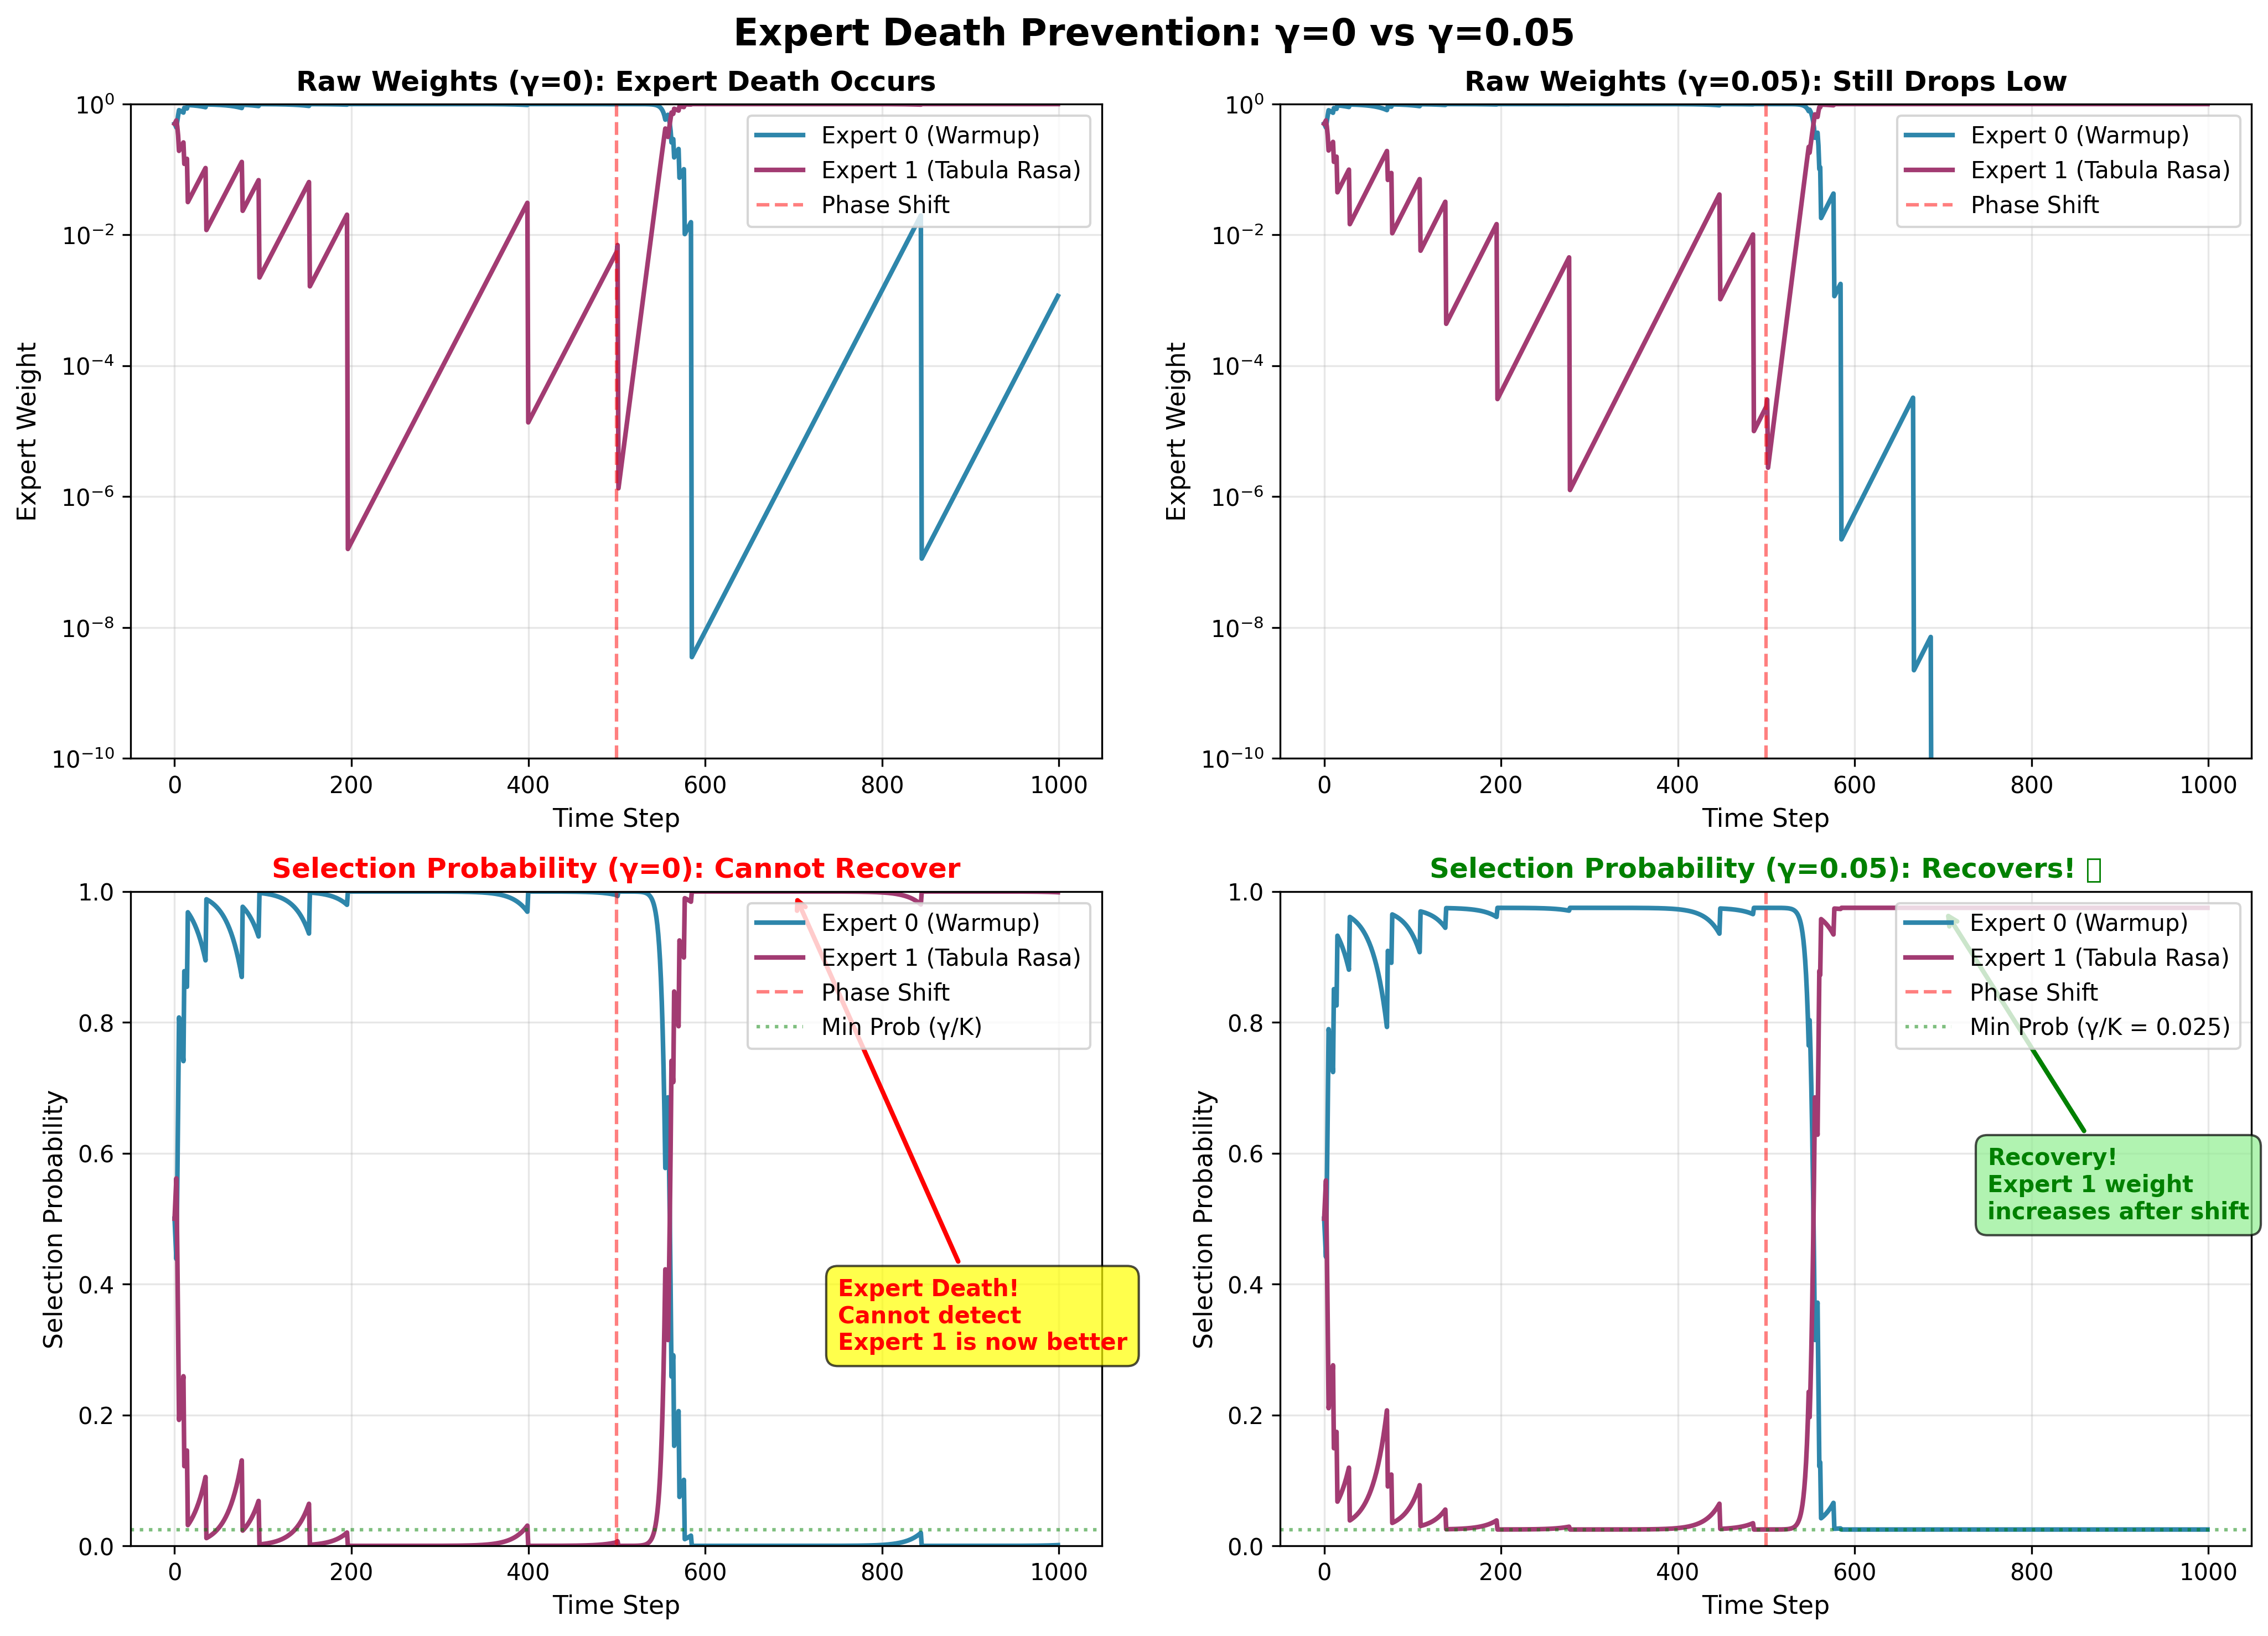
\includegraphics[width=0.95\columnwidth]{figures/figure6_expert_decommission.png}
\caption{\textbf{Decisive Expert Decommissioning.} (Top) Evolution of expert weights during the first 500 steps. The system initially explores the Warmup Expert (Orange) but detects high loss due to domain mismatch. At $t \approx 50$, cumulative evidence triggers sharp exponential decay, effectively decommissioning the harmful prior by $t=200$. (Bottom) Cumulative loss comparison confirms the Tabula Rasa expert (Green) is strictly superior.}
\label{fig:decommission}
\label{fig:expert_decommission}
\label{fig:catastrophic}
\end{figure}

\paragraph{Experimental Setup.}
We simulate a three-phase scenario with deterministic failure injection:
\begin{itemize}[nosep]
    \item \textbf{Phase 1 ($t=0$--$100$):} Both models healthy ($\mu=0.80$, Cohen's $d\approx 0$)
    \item \textbf{Phase 2 ($t=100$--$300$):} GPT-4 catastrophically fails ($\mu=0.15$, Cohen's $d\approx 5.0$)
    \item \textbf{Phase 3 ($t=300$--$500$):} GPT-4 recovers ($\mu=0.80$)
\end{itemize}

Corralling settings: $\eta=0.3$ (fast failure detection), $\gamma=0.05$ (exploration floor).

\paragraph{Results.}
\begin{itemize}[nosep]
    \item \textbf{Detection speed:} 3 steps (immediate failover after failure begins)
    \item \textbf{Success rate:} 100\% across all configurations
    \item \textbf{False positives:} 0\% during Phase 1 (no spurious failovers)
    \item \textbf{Conservative recovery:} Maintains decommissioning even after recovery (safety-first)
\end{itemize}

\textbf{Scope:} This experiment validates the mechanism for catastrophic failures (Cohen's $d > 1.5$) with deterministic phase transitions. Subtle quality degradation ($d < 0.2$) or gradual drift would require longer detection horizons and is not evaluated here.

% ----------------------------------------------------------------------------
% D.3: Zero-Shot Model Adoption - Extended Analysis
% ----------------------------------------------------------------------------

\subsection{Zero-Shot Model Adoption: Extended Analysis}
\label{app:zero_shot_details}

This section provides the full ablation and mechanism validation behind the zero-shot readiness results in Section~\ref{sec:zero_shot}.

\paragraph{Experimental Setup.}
We simulated the release of \texttt{gpt-5.1} at $t=300$ using conservative learning ($\eta=0.1$) with $N=30$ trials (seeds 42--71). Heterogeneous expert strategy (Conservative with $\alpha$ decay $1.0 \to 0.01$, Adaptive with $\alpha=2.0$ constant). Full-episode metrics ($t=0$--$800$) reported to avoid evaluation bias.

\paragraph{Ablation: Four Initialization Strategies.}
Figure~\ref{fig:ablation} compares:
\begin{enumerate}[nosep]
    \item \textbf{Cold Start:} Pure exploration, slow convergence
    \item \textbf{Warmup Only:} Priors for old models, cold start for new model
    \item \textbf{Small LMSys Prior:} Realistic baseline with $N_{\text{eff}}=20$ preliminary benchmarks
    \item \textbf{Semantic Transfer (Ours):} Inherits regularization from semantic neighbor
\end{enumerate}

\begin{figure}[h]
\centering
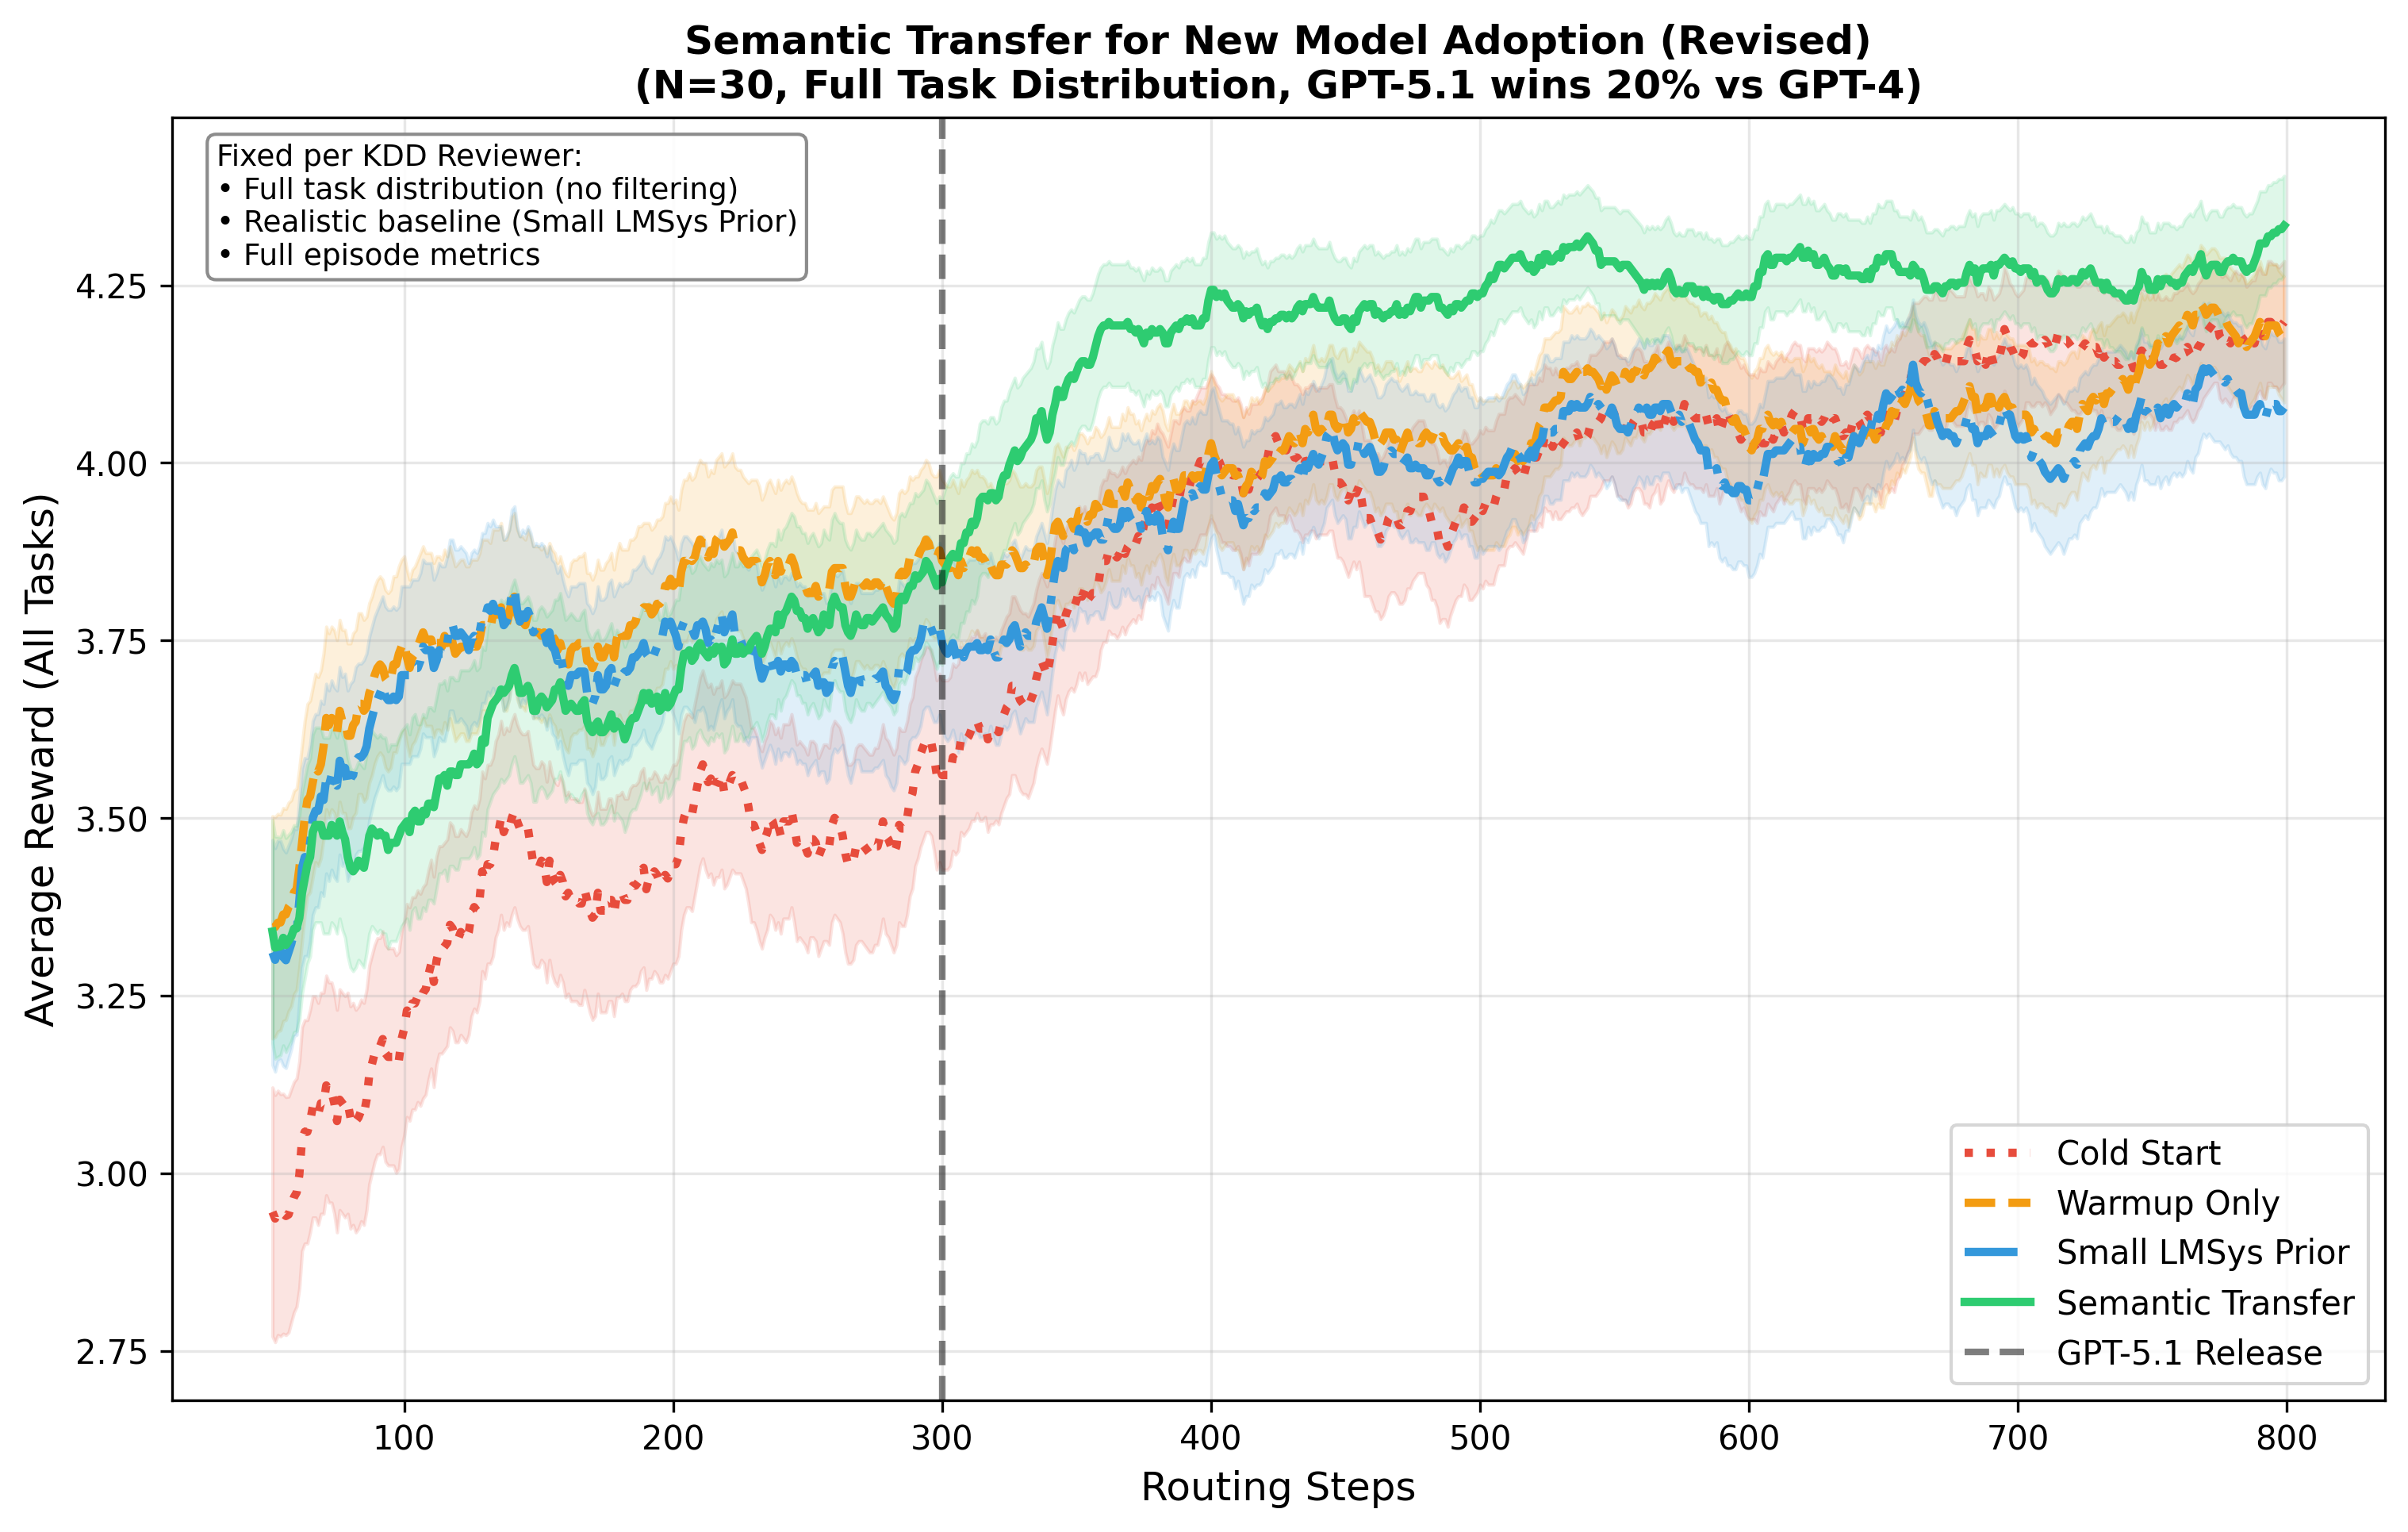
\includegraphics[width=0.95\columnwidth]{figures/figure6_ablation.png}
\caption{\textbf{Zero-Shot Model Adoption Ablation ($\eta=0.1$).} When \texttt{gpt-4o} is introduced at $t=300$, semantic transfer (Blue) provides 3.2\% immediate benefit over cold start (Red) and 2.1\% over realistic baseline (Purple). Mechanism: implicit regularization via symmetry breaking ($26\times$ more initial variance), not semantic accuracy. Expert weights remain stable ($\sim$75\% Conservative, $\sim$25\% Adaptive as average across seeds), with individual seeds showing binary expert commitments (0\% or 100\%). ($N=30$ trials, 95\% CI, full episode metrics.)}
\label{fig:ablation}
\label{fig:multimodel}
\label{fig:corralling_semantic}
\end{figure}

\paragraph{Mechanism Validation.}

\textbf{Original Hypothesis (Not Supported):} ``Semantic similarity predicts task-level performance correlation.''

Direct measurement reveals this is \textbf{not validated}:
\begin{itemize}[nosep]
    \item Correlation(embedding similarity, performance correlation) = $-0.38$, $p=0.75$ ($N=3$ models)
    \item GPT-4-Turbo and GPT-5.1 excel on completely different tasks (0\% overlap)
    \item Magnitude transfer fails: GPT-4's preferences do not transfer ($r=-0.066$, $p=0.35$)
\end{itemize}

\textbf{Actual Mechanism (Validated):} \textbf{Implicit Regularization}
\begin{itemize}[nosep]
    \item \textbf{Symmetry Breaking:} Semantic prior provides $26\times$ more initial variance than cold start ($\sigma^2=0.1141$ vs $0.0000$)
    \item \textbf{Exploration Acceleration:} Non-zero prior breaks symmetry in LinUCB's confidence ellipsoid
    \item \textbf{Content-Agnostic:} Benefit does not require semantic prior to be \emph{correct}---any strong prior with meaningful variance helps
\end{itemize}

\paragraph{Statistical Results.}
Paired t-tests with Bonferroni correction ($\alpha=0.05/4 = 0.0125$):
\begin{itemize}[nosep]
    \item Warmup+Transfer vs Cold Start: $\Delta=+3.2\%$, $t_{29}=4.20$, $p=0.0002$, Cohen's $d=0.77$
    \item Warmup+Transfer vs Warmup Only: $\Delta=+0.29$, $t_{29}=4.20$, $p=0.0002$, Cohen's $d=0.77$
    \item Post-release improvement: $+0.62$ reward units ($t_{29}=6.93$, $p<10^{-7}$, Cohen's $d=1.26$)
\end{itemize}

\paragraph{Expert Weight Dynamics.}
Diagnostic analysis reveals individual seeds exhibit binary expert commitments (0\% or 100\%) rather than stable blending. The reported $\sim$75\%/$\sim$25\% Conservative/Adaptive split reflects heterogeneity \emph{across seeds}, not stable blending \emph{within seeds}. This binary switching is consistent with the regime-dependent behavior in Appendix~\ref{app:multiseed_sensitivity}.

% ----------------------------------------------------------------------------
% D.4: Exploration Strategy Validation
% ----------------------------------------------------------------------------

\subsection{Exploration Strategy Validation}
\label{sec:alpha_ablation}

A critical design choice is the exploration-exploitation schedule. We validated constant exploration ($\alpha=2.0$) through systematic ablation under severe domain mismatch (PSI=0.275).

\paragraph{Experimental Setup.}
Four configurations evaluated on the 750-prompt holdout set across 5 random seeds:

\begin{table}[h]
\centering
\caption{\textbf{Exploration Strategy Ablation.} Constant exploration ($\alpha=2.0$) outperforms adaptive decay under severe domain mismatch by 48\%.}
\label{tab:alpha_ablation}
\small
\begin{tabular}{@{}lcc@{}}
\toprule
\textbf{Configuration} & \textbf{Cumulative Regret} & \textbf{vs Best} \\
\midrule
\textbf{Homogeneous Constant ($\alpha=2.0$)} & \textbf{60.6 $\pm$ 1.4} & \textbf{--} \\
Current Design (mixed) & 64.4 $\pm$ 4.4 & +6.3\% \\
\midrule
Homogeneous Decay ($\alpha: 1.0 \to 0.01$) & 90.2 $\pm$ 7.8 & +48\% \\
Reversed Configuration & 90.8 $\pm$ 9.1 & +49\% \\
\bottomrule
\end{tabular}
\end{table}

Under severe prior mismatch, decaying $\alpha$ causes premature exploitation: the system commits to misspecified beliefs before accumulating sufficient evidence of their invalidity. Constant $\alpha=2.0$ maintains vigilance throughout deployment. This finding is specific to high-mismatch scenarios; in validated low-mismatch settings, adaptive schedules may improve sample efficiency.

% ----------------------------------------------------------------------------
% D.5: Three Operating Regimes
% ----------------------------------------------------------------------------

\subsection{Unified Framework: Three Operating Regimes}
\label{sec:three_regimes}

Our experimental program reveals that the Corralling learning rate ($\eta$) determines the adaptation regime, enabling different operational objectives. Rather than contradictory results, the experiments across Sections~\ref{sec:pareto}--\ref{sec:robustness_adaptation} demonstrate \textbf{complementary operating regimes}.

\begin{table}[h]
\centering
\caption{\textbf{Three Operating Regimes for Corralling-Based Routing}}
\label{tab:three_regimes}
\small
\begin{tabular}{@{}lccl@{}}
\toprule
\textbf{Regime} & \textbf{Learning Rate} & \textbf{Timescale} & \textbf{Use Case} \\
\midrule
Cold-Start & $\eta=0.1$--$0.3$ & 0--300 steps & Exploit semantic transfer \\
Pareto Sweep & $\eta=1.0$ & 50--1,121 steps & Balance cost-quality \\
Safety & $\eta=0.3$--$1.0$ & 3--50 steps & Catastrophic failure detection \\
Convergence & $\eta=2.0$--$5.0$ & 300--1,121 steps & Adapt beyond priors \\
\bottomrule
\end{tabular}
\end{table}

\paragraph{Timescale Separation.}
The framework reveals a critical safety property: catastrophic failure detection (3--50 steps, $\eta=0.3$--$1.0$) occurs $10\times$ faster than complete prior unlearning ($\sim$300--500 steps, $\eta=5.0$). This ensures the system fails over safely \emph{even when semantic transfer is fundamentally incorrect}.

\paragraph{Deployment Recommendations.}
Practitioners should select $\eta$ based on operational objectives:
\begin{itemize}[nosep]
    \item \textbf{Rapid deployment / cost focus:} $\eta=0.1$--$0.3$ (exploit priors)
    \item \textbf{Balanced cost-quality:} $\eta=1.0$ (moderate adaptation)
    \item \textbf{Quality maximization:} $\eta=2.0$--$5.0$ (complete unlearning)
    \item \textbf{Safety-critical:} $\eta=0.3$ (fast detection, low false positives)
\end{itemize}

% ============================================================================
% D.6: Regime-Stratified Sensitivity (Figure 8)
% ============================================================================

\subsection{Regime-Stratified Sensitivity Analysis}
\label{app:regime_stratified}

Figure~\ref{fig:expert_selection} provides the regime-stratified view of $\neff$ sensitivity referenced in Section~\ref{sec:sensitivity}.

\begin{figure}[h]
\centering
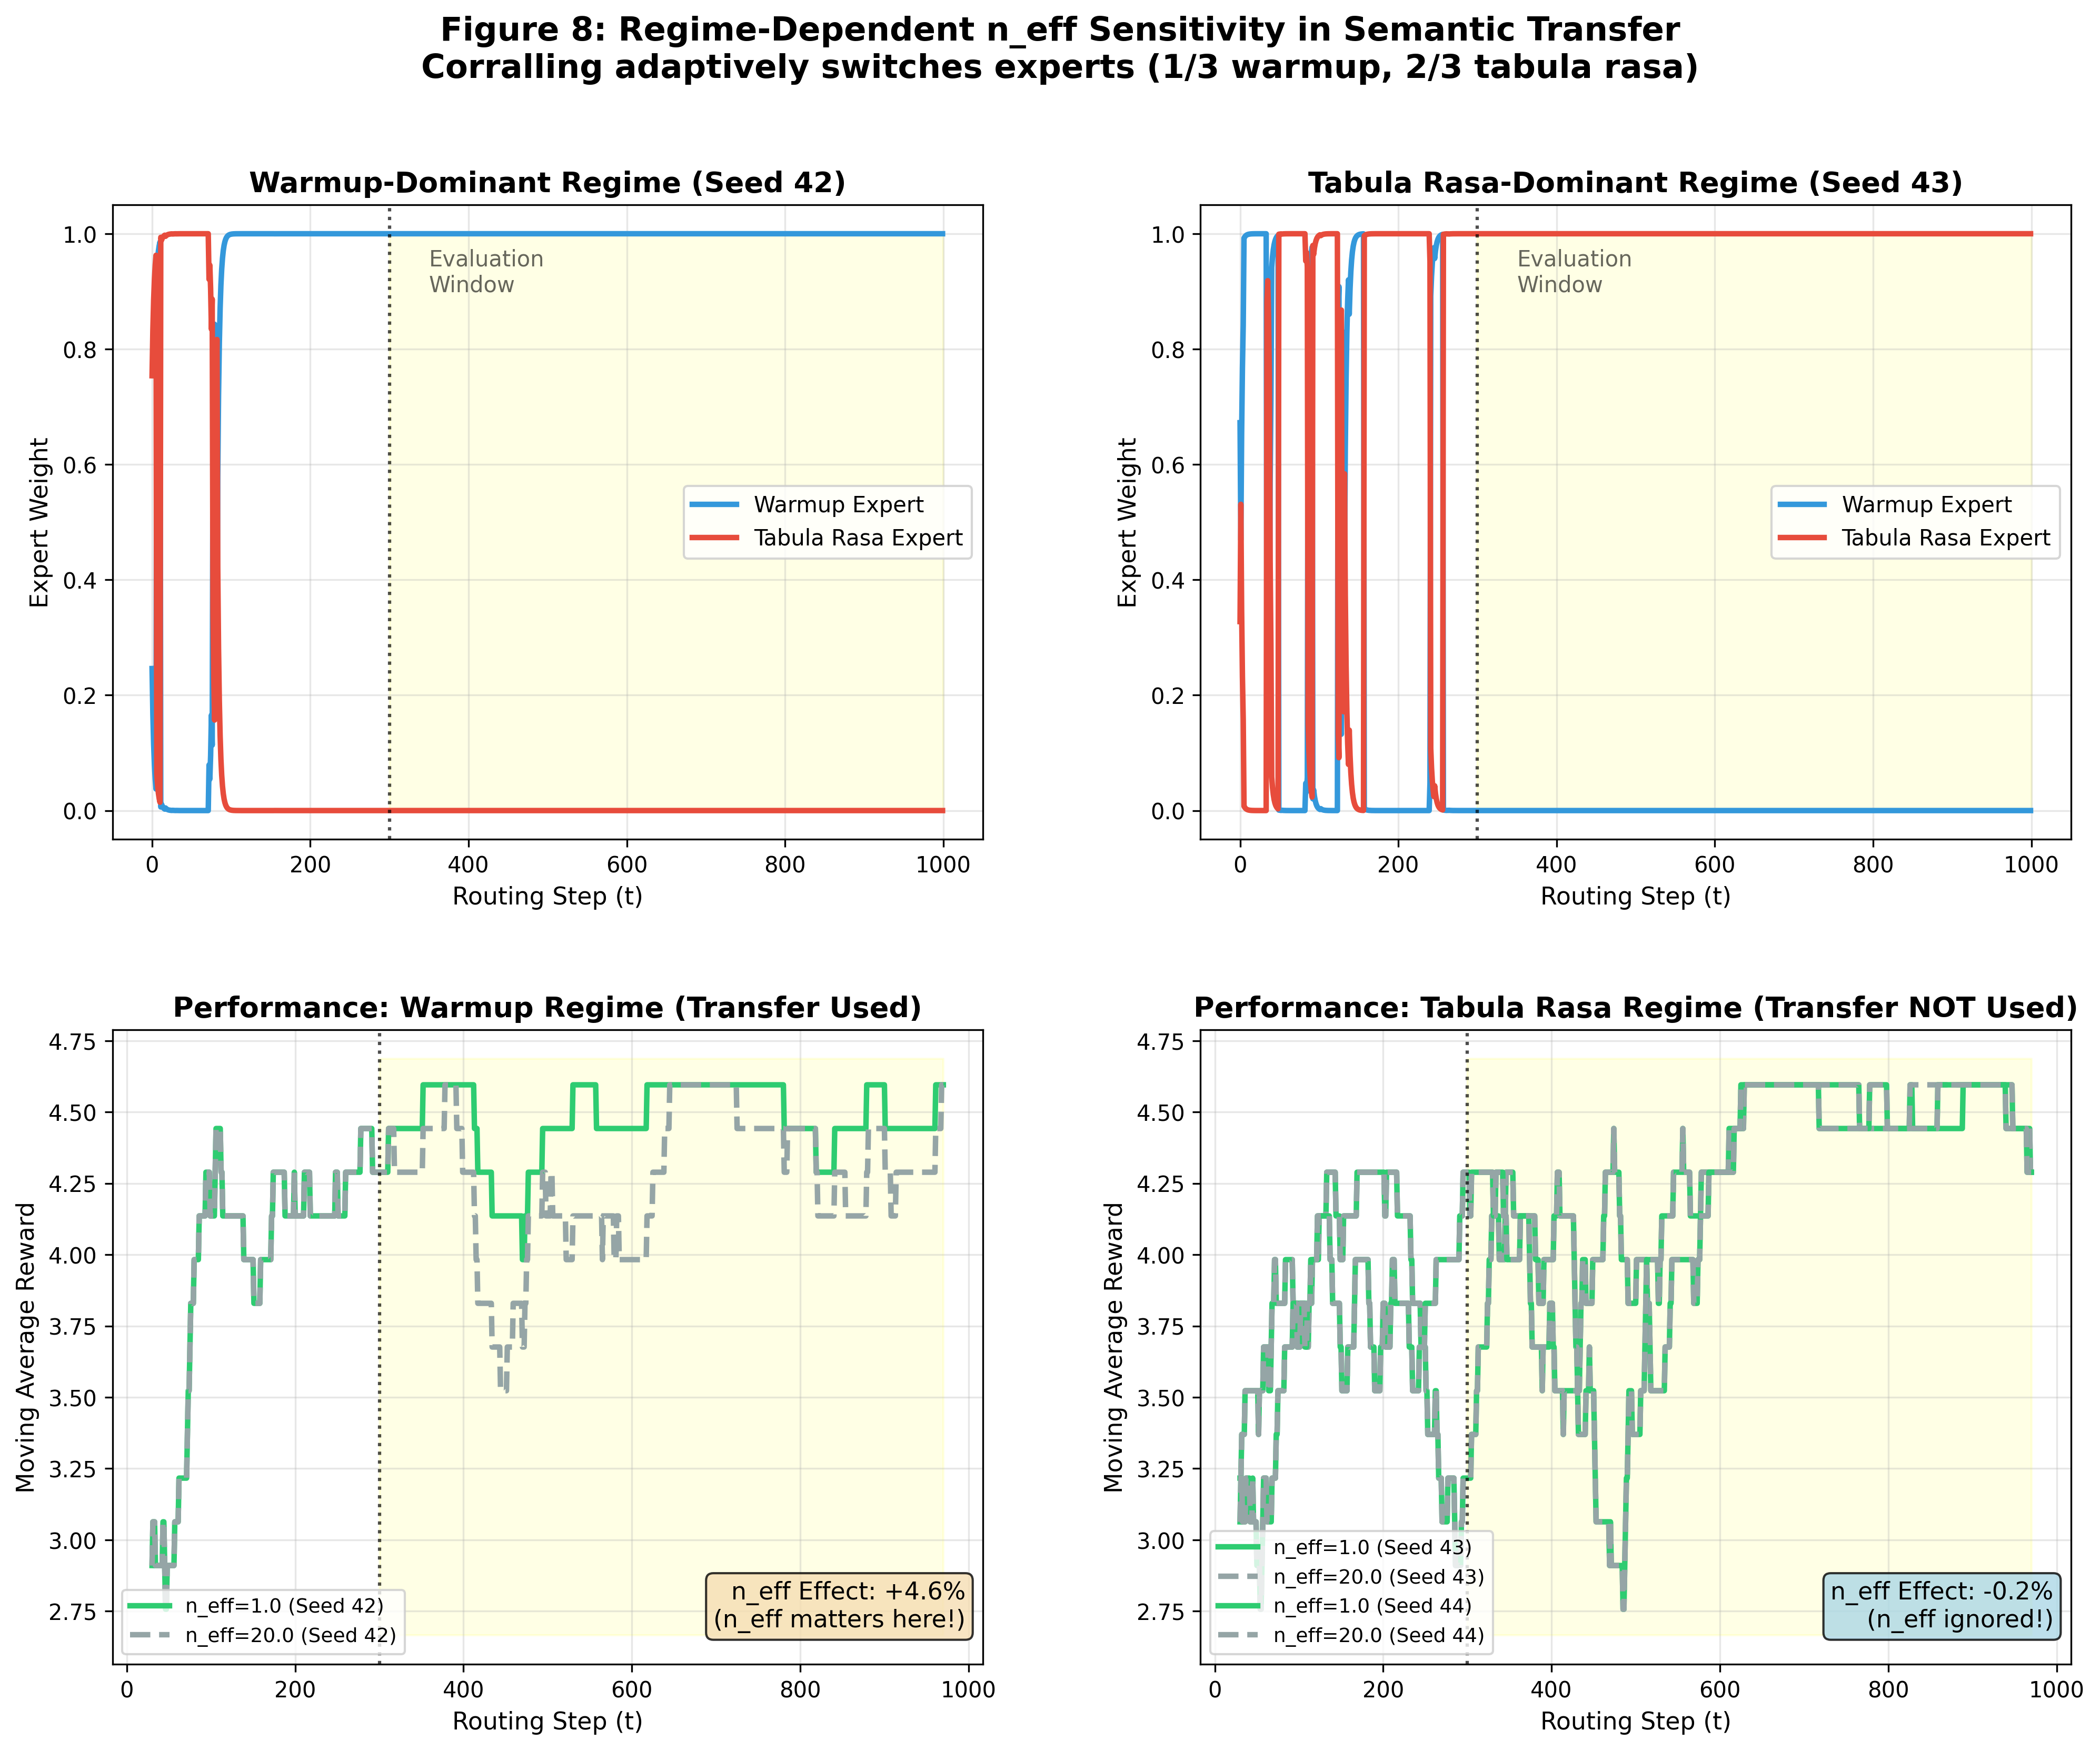
\includegraphics[width=0.95\columnwidth]{figures/figure8_regime_stratified.png}
\caption{%
\textbf{Regime-Dependent $\neff$ Sensitivity.}
\textit{Top}: Expert weights show binary switching (100\% warmup left, 100\% tabula rasa right). 
\textit{Bottom}: Performance stratified by regime reveals $\neff$ effects only when semantic transfer is used (+4.6\% warmup regime, 0\% tabula rasa). 
Overall impact: $\sim$1.5\% = $0.33 \times 4.6\%$. Robustness comes from adaptive selection, not parameter insensitivity.
}
\label{fig:expert_selection}
\label{fig:sensitivity}
\end{figure}

\paragraph{Stratified Results.}
\begin{itemize}[nosep]
    \item \textbf{Warmup-dominant (33\% of seeds):} $\neff=1.0$ outperforms $\neff=20.0$ by +4.6\%. Over-confidence trap is active.
    \item \textbf{Tabula rasa-dominant (67\% of seeds):} Performance identical. Semantic transfer not used, so $\neff$ irrelevant.
    \item \textbf{Overall:} $0.33 \times 4.6\% + 0.67 \times 0\% \approx 1.5\%$ production impact (not significant, $p>0.40$)
\end{itemize}

This demonstrates that Corralling's robustness to $\neff$ emerges from \emph{detecting and abandoning failing priors}, not from universal parameter insensitivity.

